\documentclass[10pt,a4paper]{article}
\usepackage[utf8]{inputenc}
\usepackage{amsmath}
\usepackage{amsfonts}
\usepackage{amssymb}
\usepackage{listings}
\usepackage{graphicx}
\usepackage{caption}
\usepackage{subcaption}
\usepackage{float}
\lstset{showstringspaces=false,
		breaklines=true,
		postbreak=\raisebox{0ex}[0ex][0ex]{\ensuremath{\hookrightarrow\space}}}
    	
\begin{document}
\title{Intelligent Systems Assignment 3}
\author{Wessel Becker (1982362) \& Sander ten Hoor (2318555)}
\maketitle

\section{Matlab Code}
The following code was created for edge detection and boundary detection.

\subsection{simpleDifferentiation.m}
\lstinputlisting[language=Matlab]{./edgedetection/simpleDifferentiation.m}

\subsection{robert.m}
\lstinputlisting[language=Matlab]{./edgedetection/robert.m}

\subsection{sobel.m}
\lstinputlisting[language=Matlab]{./edgedetection/sobel.m}

\subsection{prewitt.m}
\lstinputlisting[language=Matlab]{./edgedetection/prewitt.m}

%\subsection{cannyEdgedetection.m}
%\lstinputlisting[language=Matlab]{./edgedetection/cannyEdgedetection.m}

\subsection{boundaryExtraction.m}\label{list:boundaryExtraction}
\lstinputlisting[language=Matlab]{./edgedetection/boundaryExtraction.m}

\section{Edge Detection}
While all the results suffer from noise, the Simple Differentiation and the Roberts algorithm become nearly unrecognisable, while the others still show clear lines.

\section{Boundary Extraction}
For exercise 2.2 a simple boundary extractor was build as can be found in the code listings \ref{list:boundaryExtraction}. This very simple boundary extractor can be run with a variable threshold for hit detection. And works by first eroding anything that could be the inside of a shape by doing an erosion with a 3 * 3 structuring element with the origo in the center. This will erode any pixel tat is not surrounded by other accepted pixels but is accepted, or in other words the boundaries. If we then subtract this image from our original binary image of accepted values we are left with the pixels we eroded before or in other words the boundaries as seen in \ref{fig:}.


\section{Work done}

\section{Edge Detection images}
\subsection{Simple Differentiation}
\begin{figure}[H]
  \centering
  
  \begin{subfigure}{.5\textwidth}
    \centering
    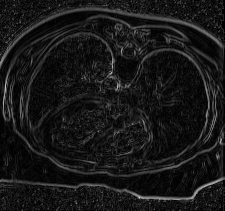
\includegraphics[width=.9\textwidth]{./edgedetection/images/sd_no_noise}
    \caption{Simple Differentiation, no noise}
    \label{fig:sd_no_noise}
  \end{subfigure}%
  \begin{subfigure}{.5\textwidth}
    \centering
    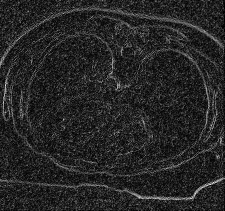
\includegraphics[width=.9\textwidth]{./edgedetection/images/sd_001_noise}
    \caption{Simple Differentiation, Gaussian noise with variance = 0.001}
    \label{fig:sd_001}
  \end{subfigure}\\%
  \begin{subfigure}{.5\textwidth}
    \centering
    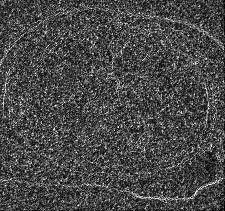
\includegraphics[width=.9\textwidth]{./edgedetection/images/sd_005_noise}
    \caption{Simple Differentiation, Gaussian noise with variance = 0.005}
    \label{fig:sd_005}
  \end{subfigure}%
  
\end{figure}

\subsection{Roberts}
\begin{figure}[H]
  \centering
    \makebox[\textwidth]{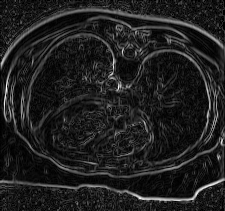
\includegraphics{./edgedetection/images/robert_no_noise}} \\
  \caption{Roberts, no noise}
  \label{fig:robert_no_noise}
\end{figure}
\begin{figure}[H]
  \centering
    \makebox[\textwidth]{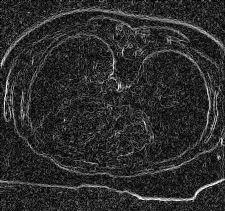
\includegraphics{./edgedetection/images/robert_001_noise}} \\
  \caption{Roberts, Gaussian noise with variance = 0.001}
  \label{fig:robert_001}
\end{figure}
\begin{figure}[H]
  \centering
    \makebox[\textwidth]{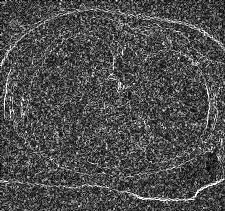
\includegraphics{./edgedetection/images/robert_005_noise}} \\
  \caption{Roberts, Gaussian noise with variance = 0.005}
  \label{fig:robert_005}
\end{figure}

\subsection{Sobel}
\begin{figure}[H]
  \centering
    \makebox[\textwidth]{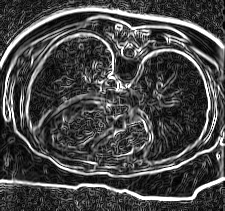
\includegraphics{./edgedetection/images/sobel_no_noise}} \\
  \caption{Sobel, no noise}
  \label{fig:sobel_no_noise}
\end{figure}
\begin{figure}[H]
  \centering
    \makebox[\textwidth]{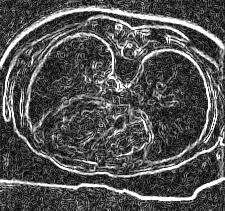
\includegraphics{./edgedetection/images/sobel_001_noise}} \\
  \caption{Sobel, Gaussian noise with variance = 0.001}
  \label{fig:sobel_001}
\end{figure}
\begin{figure}[H]
  \centering
    \makebox[\textwidth]{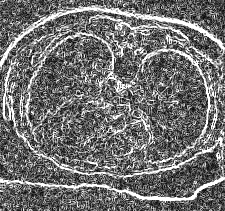
\includegraphics{./edgedetection/images/sobel_005_noise}} \\
  \caption{Sobel, Gaussian noise with variance = 0.005}
  \label{fig:sobel_005}
\end{figure}

\subsection{Prewitt}
\begin{figure}[H]
  \centering
    \makebox[\textwidth]{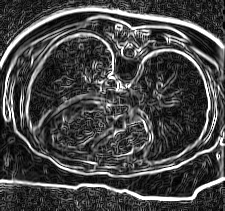
\includegraphics{./edgedetection/images/prewitt_no_noise}} \\
  \caption{Prewitt, no noise}
  \label{fig:prewitt_no_noise}
\end{figure}
\begin{figure}[H]
  \centering
    \makebox[\textwidth]{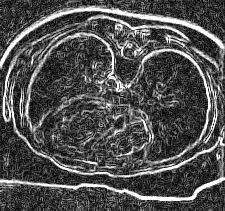
\includegraphics{./edgedetection/images/prewitt_001_noise}} \\
  \caption{Prewitt, Gaussian noise with variance = 0.001}
  \label{fig:prewitt_001}
\end{figure}
\begin{figure}[H]
  \centering
    \makebox[\textwidth]{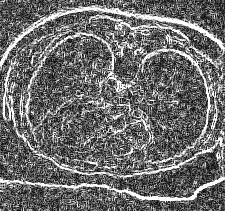
\includegraphics{./edgedetection/images/prewitt_005_noise}} \\
  \caption{Prewitt, Gaussian noise with variance = 0.005}
  \label{fig:prewitt_005}
\end{figure}
\end{document}